%\documentclass[SparseCoding.tex]{subfiles}
\section{\textit{Sparseland}}

Modeling data play a central role in signal processing and machine learning. Sparse representation model also refers as \textit{Sparseland} \cite{8398588},  suggests a description of every signal as sparse linear combinations of basic elements called \textit{atoms}, which come from a redundant matrix called a \textit{dictionary}. Redundant matrix means that we have more atoms than the size of the corresponding signal. \\
The Sparseland model became one of the most important modelizations in image processing, and more generally in signal processing. Its give state-of-the-art results in a wide variety of tasks: Denoising, inpainting, image separation, deblurring,\dots\\
There is one fundamental property on which this theory is based, the same property which allows us to compress a signal, to denoise, enhance a degraded signal, \dots. All meaningful data sources (i.e signal) are structured.\\
Each source of information: image, audio, video, 3D object (meshes or points cloud),  text, financial time series, data on a graph,\dots  have an inner structure that is unique to them which can be characterized in various ways and allow redundancy.\\

The first signs of \textit{Sparseland} appear in the 1990s with the greedy and relaxed pursuit algorithm \cite{258082,305222} and the introduction of dictionary learning \cite{Olshausen97sparsecoding}.

\subsection*{The idea behind \textit{Sparseland}}
The first step in \textit{Sparseland} is to find (i.e learn) a dictionary with a relevant set of atoms (this step is called \textbf{Dictionary Learning}). Then the model assumption is that every incoming signal could be represented as a linear combination of only a few atoms from the dictionary (this step is called \textbf{Sparse Coding}).\\ \vspace{-0.4cm}
\begin{center}
\fbox{\begin{varwidth}{\textwidth}
\centering
\hspace{-5.5cm}\textbf{Definition:} Sparse \\ \vspace{0.2cm} \textit{ Occurring at widely spaced intervals, not thick or dense.}
\end{varwidth}}
%\fbox{\textbf{Definition:} \\Sparse:
%\textit{ Occurring at widely spaced intervals, not thick or dense.}}
\end{center}\vspace{0.4cm}
Unlike decomposition based on principal component analysis, \textit{Sparseland} does not impose that learned representation to be orthogonal, allowing more flexibility to adapt the representation to the signal.
\\
The idea of finding new representations of an input signal is not new. Signal processing's scientists already use this approach with predefined dictionaries instead of a learned one, for example, wavelets transform or Fourier transform. With a learned dictionary, we can expect to get more relevant information about the inner structure of the signal. For that reason, we can expect better performances in a wide range of applications.

\section{Mathematical formulation}


 \begin{figure}[h]
 \centering
 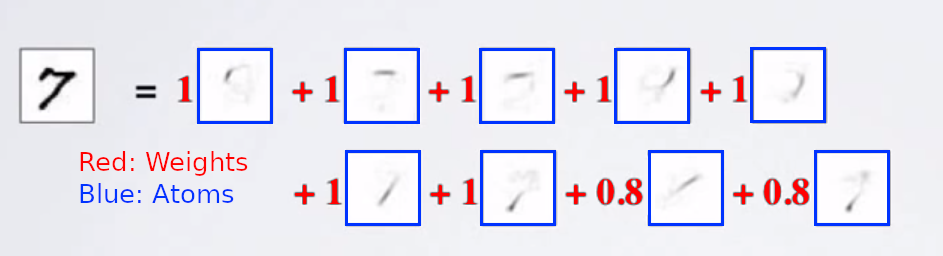
\includegraphics[scale=0.5]{spacecoding_12.png}
 % spacecoding_1.png: 943x256 px, 96dpi, 24.95x6.77 cm, bb=0 0 707 192
 \caption{Example of Sparse Coding reconstruction}
 \label{fig:exemple}
\end{figure}

Consider a signal $x_i \in \R^m$ in a set of signal $X = [x_1, x_2, \ldots, x_n] \in \R^{m \times n}$ ( generally $n$ is large and $m$ is small: $n >> m$), the aim of this method is to find a linear combination of overcomplete basis elements $D = [d_1, d_2, \ldots, d_k]$ under sparsity constraints which reconstruct the input signal (see  an example at figure \ref{fig:exemple}), overcomplete dictionary mean that $k > m$:
\begin{center}
 $x_i = D \gamma_i$
 \\ With $\gamma_i$ the sparse coefficients of the sparse decomposition for the signal $x_i$
\end{center}

The traditional way to get $\gamma_i$ is to optimize the empirical cost function.
\begin{center}
 $f_n(D) = \frac{1}{n} \sum_{i=1}^{n} l (x_i,D)$
\end{center}
Where $l$ is the cost function which is small where D is good for representing the signal. Usually, we use :
\begin{center}
 $l(x_i,D) =   \min\limits_{\gamma_i} \frac{1}{2} \underset{Squared\ error}{\underbrace{\| x_i - D \hspace{3px} \gamma_i \|_2^2}} + \lambda \underset{Sparsity\ term}{\underbrace{ \|\gamma_i \|_0}}$
\end{center}
Note that the cost function has two terms, which fight each other.  The first term corresponds to the squared error, while that the second term corresponding to the sparsity of the weight vector. $\lambda$ is a positive constant which controls the importance of the sparse term relative to the square error term. \\
The norm of all columns of D must be equal or less than 1  , otherwise, D could grow big while $\gamma$ becomes small to satisfy the prior.\\
This problem is also known as a \textit{basic pursuit}  or the  \textit{Lasso}. However, it is important to notice that the problem isn't convex and his optimization is NP-complete (due to the $l_0$ norm). Fortunately, it is well known that for kind of problem use $l_1$ norm instead of $l_0$ norm yields a sparse solution for $\gamma_i$.\\
Then the optimization problem can be rewritten as:
\begin{center}
 $\min\limits_{D} \frac{1}{n} \sum_{i=1}^{n}  \min\limits_{\gamma_i} \frac{1}{2} \| x_i - D \hspace{3px} \gamma_i \|_2^2 + \lambda \|\gamma_i \|_1$
\end{center}
Before presenting our experimentations we will explain how traditional Sparse Coding works. In particular, how this method learns redundant properties and patterns in a signal set. This is the learning phase.
\newpage
\section{Learning step}
A natural approach to solve this optimization problem is to alternate between the optimization of $D$ and $\gamma$, minimize over one while keeping the other one fixed.\\
\begin{algorithm}
 \label{algo:algo1}

 \caption{Learning step}
 \begin{algorithmic}
 \REQUIRE X the input signal
    \STATE $D_0$ initilized randomly, $\gamma$  is a zeros matrix
    \WHILE{D and $\gamma$ not converged}
        \STATE Fix D
        \STATE Find $\gamma$ \hspace{0.7cm} \textit{/* Sparse Coding step */}   (1)
        \STATE Fix $\gamma$
        \STATE Find D \hspace{0.7cm} \textit{/*Dictionary Learning  */} (2)
    \ENDWHILE
 \end{algorithmic}

\end{algorithm}

% 
% \paragraph{Idea} Sparse dictionary learning is a representation learning method which aims at finding a sparse representation of the input data (in form of a linear combination of basic elements (called Atoms). The idea of using a learned dictionary instead of a predefined one is based on wavelets.  The sparse learned models has recently led to state-of-the-art result for denoising, classification,...
% %UNSPERVISED LEARNING=========================================================+
% \paragraph{Unsupervised learning} Only use the inputs $x^{(t)}$ ( $X = [x_1,....,x_n]$ in $\R^{m \times n}$) for learning. Automatically extract meaningful features of our data, leverage the availability of unlabeled data and add a data-dependent regularize to trainings.\\
% 
% Sparse coding is one of the methods used for unsupervised learning  (like restricted Boltzmann machines and autoencoders).\\
% The idea behind sparse coding is: For each $x^{t}$ find a latent representation $\gamma^{t}$ such that:
% \begin{itemize}
%  \item[$\bullet$] It is sparse: the vector $\gamma^{t}$ has many zeros (only few nonzero elements)
%  \item[$\bullet$] We can reconstruct the original input $x^{(t)}$ as well as possible.
% \end{itemize}
% That mean, more formally:\\
% 
% %Formulation du problème=============================
% \begin{center}
%  $\min\limits_{D} \frac{1}{T} \sum_{t=1}^{T}  \min\limits_{\gamma^{(t)}} \frac{1}{2} \| x^{(t)} - D \hspace{3px} \gamma^{(t)} \|_2^2 + \lambda \|\gamma^{(t)} \|_1$\\
% \end{center}
% 
%  %Explicaiton de la formulation=========================
%  \begin{itemize}
%  \item[$\bullet$] D is a matrix of weights, usually refer to that matrix as a dictionary matrix (containt atoms) with $D \in  \R^{m \times k}$ ( k the number of atoms)
%   \item[$\bullet$] $\| x^{(t)} - D \hspace{3px} \gamma^{(t)} \|_2^2 $ is the reconstruction error
%   \item[$\bullet$]$ D \hspace{3px} \gamma^{(t)}$ is the reconstruction of $\hat{x}^{(t)}$
%   \item[$\bullet$]$\|\gamma^{(t)} \|_1$ is the sparsity penalty (more 0 in h we have, better it is)
%  \end{itemize}
% This two objectives fight each other. But it still a optimization problem (cf min), and we'll try to optimize it for each training example $x^{(t)}$. This is why we have a sum over all the training examples.
% \newline
% 
% %Contraintes sur D======================================
% \indent We also constrain the columns of D to be of norm 1 (otherwise, D could grow big while $\gamma^{(t)}$ becomes small to satisfy the prior). And sometimes the columns are constrained to be no greather than 1.\\
% 
% However, $\gamma^{(t)}$ is now a complicated function of $x^{(t)}$:\\
% Encoder is the minimization $\gamma(x^{(t)}) = arg\min\limits_{\gamma^{(t)}}= \frac{1}{2} \| x^{(t)} - D \hspace{3px} \gamma^{(t)} \|_2^2 + \lambda \|\gamma^{(t)} \|_1$, so the optimization problem is more complicated than a simple non linear problem.\\
% The idea to solve this minimization problem is \cite{NIPS2006_2979}
% 
% \begin{lstlisting}[language=Python,frame=single]
% while D not_converged :
%     Fix D
%     Minimize alpha     (1) // Sparse Coding step
%     Fix alpha
%     Minimize D           (2) // Update Dictionary step
% \end{lstlisting}
% 
% But there are some improvement like K-SVD algorithm \cite{KSVD}, which compute column by column a SVD computation over the relevant examples.
% %DICTIONARY==================================================================+  
% \paragraph{Dictionary}
% We can also write $\hat{x}^{(t)} = D\hspace{3px} \gamma(x^{(t)}) \displaystyle\sum_{\substack{k s.t.\\ \gamma(x^{(t)})_k\neq 0}}  D.,_k \gamma(x^{(t)} )_k$
% \begin{figure}[h]
%  \centering
%  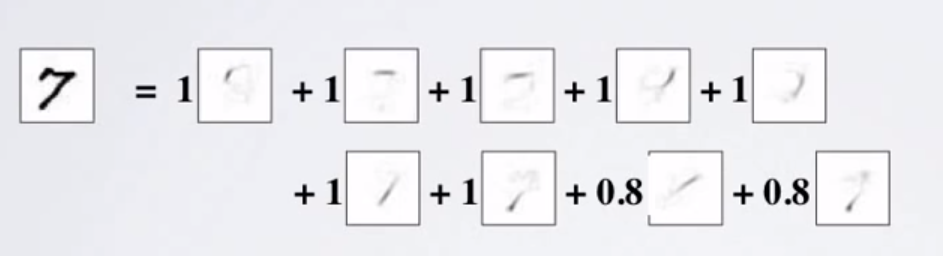
\includegraphics[scale=0.5]{spacecoding_1.png}
%  % spacecoding_1.png: 943x256 px, 96dpi, 24.95x6.77 cm, bb=0 0 707 192
%   \caption{Example of reconstruction using sparse coding}
% \end{figure}
% 
% The images refer to $D.,_k$ (columns of D wich are not equals to 0) and the factor (1 or 0.8 in this case) refer to $\gamma(x^{(t)} )_k$
% \\We also refer to D as the dictionary:
% \begin{itemize}
%  \item[$\bullet$]in certain applications, we know what dictionary matrix to use
%  \item[$\bullet$]often however, we have to learn it
% \end{itemize}
% 
% In general we have $k<<n$ . But we can use an overcomplete dictionary with $k > m$.
% 
%\end{document}
